%!TEX root = ./../../springer-mono-format/book.tex
%!TEX root = ./../../thesis-trier.tex

Here, we state and prove the following.

\begin{enumerate}
	
\item \DFASW is \LOGSPACE-complete even for partially ordered unary input automata
and a single input word (\cref{prelim:prop:finite_list_sync_word-hardness,prelim:thm:finite_list_sync_word}).
	
\item \DFAST is \NL-hard even for a fixed binary alphabet (\cref{prelim:prop:sync_NL_complete}).
 The proof is a simplified version of a 
 construction given by Hoffmann~\cite[Thm.~5]{DBLP:journals/tcs/Hoffmann21},
 which is similar to a construction
 from Holzer \& Jacobi~\cite[Lem.~14]{HolzerJ18}
 but uses a binary instead of a ternary alphabet.
 The proof
 from Volkov~\cite[Prop.~2.2, due to Sreejith]{Volkov22}
 uses only a binary alphabet as well,
 and is also similar to the proof given here.
 In \cref{prelim:complexity:prop:maximum,prelim:complexity:prop:maximal} 
 we also give the related results
 that checking whether a state is a maximum or maximal for $\lereach$
 in an automaton is \NL-complete.
 
\item \DFAS, \DFAST, and \DFASS 
 are all \NL-complete, even for a fixed binary alphabet that is not part of the input (\cref{prelim:complexity:general_aut_sync}).
 
\item \PSPACE-completeness of \SFS, \SIS, \DFAINT, \DST, \ST, \REACH, and \REACHF (\cref{prelim:thm:ST-PSPACE,prelim:thm:binary_pspace_problems}).
\end{enumerate}

\begin{proposition}
	\label{prelim:prop:finite_list_sync_word-hardness}
	\DFASW is \LOGSPACE-hard even for a single word as parameter
	and unary partially ordered automata. 	
\end{proposition}
\begin{proof}
	We give a reduction from \ORD,
	which is \LOGSPACE-complete by~\crefitem{prelim:thm:complexities}{prelim:thm:complexities:ORD}.
	Let $(G, v_i, v_j)$ be an input instance
	with $G = (V, E)$ and $v_i,v_j \in V$
	where $V = \{v_1, \ldots, v_n\}$
	and $E = \{ (v_i, v_{i+1}) \mid i\in \{1,\ldots,n-1\}\}$.
	We can assume $i \ne j$ and $i,j \notin \{1,n\}$.
    Note that~$v_1$ (resp.~$v_n$) is easily computable
    as the unique vertex without any ingoing (resp.~outgoing)
    vertices.  
		
	\medskip 
	\noindent\underline{Construction:} 	Set $\semiautomat{A}{V \cup \{1,\ldots,n\} \times \{v_1,v_i,v_j\}}{\{a\}}{\delta}$
	where, for $v_r \in V$, $v_s \in \{v_1,v_i,v_j\}$, $m \in  \{1,\ldots,n\}$, 
%	\[
%	\begin{array}{rl}
%		& \delta(v_r, a) \\
%		& =  \begin{cases}
%			v_{r+1}        & \text{if } r \notin \{i,j,n\}, \\
%			(0,v_r)        & \text{if } r \in \{i,j\}, \\
%			v_r            & \text{if } r = n,
%		\end{cases} 
%	\end{array} 
%	\quad 
%	\begin{array}{rcl}
%		& \delta(v_r, x) \\
%		& = & \begin{cases}
%			v_{r+1}        & \text{if } r \notin \{i,j,n\}, \\
%			(0,v_r)        & \text{if } r \in \{i,j\}, \\
%			v_r            & \text{if } r = n,
%		\end{cases} 
%	\end{array}     
%	\]
	\begin{align*}
		\delta(v_r, a) & = \begin{cases}
			v_{r+1}        & \text{if } r \notin \{i,j,n\}, \\
			(1,v_r)        & \text{if } r \in \{i,j\}, \\
			v_r            & \text{if } r = n,
		\end{cases} \\
		\delta((m, v_s), a) & = \begin{cases}
			(m+1, v_s) & \text{if } m < n, \\
			v_1        & \text{if } m = n \text{ and } s = 1, \\
			v_i        & \text{if } m = n \text{ and } s = j, \\
			v_n        & \text{if } m = n \text{ and } s = i.
		\end{cases} 	
	\end{align*}
	See Figure~\ref{fig:reductionORD} for a graphical depiction of~$\mathcal A$ for both 
	cases $i < j$ and $i > j$.
	Now, $\mathcal A$ is a unary partially ordered automaton with trap state $v_n$.
		
		
	\begin{figure}[ht]
		\centering		
		\resizebox{1.0\textwidth}{!}{%
		\begin{tikzpicture}[node distance = 4em and 2.5em, on grid, auto, ->]
				\tikzstyle{state} = [circle,fill,inner sep=1pt]
				%\node[state] (S) {Start};		
				\VertexChain{A}{1}{i}{j}{n}
				
				\path[->] (A-i) edge (A-in);
				\path[->] (A-j) edge (A-jn);
				
				\node[right = of A-n, xshift=0.5em] (transform-arrow) {\LARGE $\leadsto$};
				
				\VertexChain[transform-arrow]{B}{1}{i}{j}{n}
				
				\node[below = of B-1]   (tn-v1)     {$(n, v_1)$};
				\node[below = of tn-v1, yshift=10pt] (tn-v1dots) {$\vdots$};
				\node[below = of tn-v1dots, yshift=10pt] (t1-v1) {$(1,v_1)$};
				
				\node[above = of B-i]            (t1-vi) {$(1, v_i)$};
				\node[above = of B-n, ]          (tn-vi) {$(n,v_i)$};
				\node at ($(t1-vi)!0.5!(tn-vi)$) (t1-vidots) {$\cdots$};
				
				\node[below = of B-j]   (t1-vj)     {$(1, v_j)$};
				\node[below = of B-i]   (tn-vj)     {$(n, v_j)$};
				\node at ($(t1-vj)!0.5!(tn-vj)$) (t1-vjdots) {$\cdots$};	
				
				\path[->] (t1-v1) edge (tn-v1dots) (tn-v1dots) edge (tn-v1) (tn-v1) edge (B-1);	
				
				\path[->] (B-i) edge (t1-vi);
				\draw[->, shorten >=15pt] (t1-vi) edge (t1-vidots); 
				\path[->, shorten <=15pt] (t1-vidots) edge (tn-vi); 
				\path[->] (tn-vi) edge (B-n);
				
				\path[->] (B-j) edge (t1-vj) (t1-vj) edge (t1-vjdots) (t1-vjdots) edge (tn-vj) (tn-vj) edge (B-i);
				\path[->] (B-n) edge [loop below, looseness=65] (B-n);
		\end{tikzpicture}}
		
		\resizebox{1.0\textwidth}{!}{%
			\begin{tikzpicture}[node distance = 4em and 2.5em, on grid, auto, ->]
				\tikzstyle{state} = [circle,fill,inner sep=1pt]		
				
				\VertexChain{A}{1}{j}{i}{n}
				
				\path[->] (A-i) edge (A-in);
				\path[->] (A-j) edge (A-jn);
				
				\node[right = of A-n, xshift=0.5em] (transform-arrow) {\LARGE $\leadsto$};
				
				\VertexChain[transform-arrow]{B}{1}{j}{i}{n}
				
				\node[below = of B-1]   (tn-v1)     {$(n, v_1)$};
				\node[below = of tn-v1, yshift=10pt] (tn-v1dots) {$\vdots$};
				\node[below = of tn-v1dots, yshift=10pt] (t1-v1) {$(1,v_1)$};
				
				\node[above = of B-i, xshift=0cm]   (t1-vi) {$(1, v_i)$};
				\node[above = of B-n] (tn-vi) {$(n,v_i)$};
				\node at ($(t1-vi)!0.5!(tn-vi)$) (t1-vidots) {$\cdots$};
				
				\node[below = of B-j]   (t1-vj)     {$(1, v_j)$};
				\node[below = of B-i]   (tn-vj)     {$(n, v_j)$};
				\node at ($(t1-vj)!0.5!(tn-vj)$) (t1-vjdots) {$\cdots$};	
				
				\path[->] (t1-v1) edge (tn-v1dots) (tn-v1dots) edge (tn-v1) (tn-v1) edge (B-1);
				\path[->] (B-i) edge (t1-vi) (t1-vi) edge (t1-vidots) (t1-vidots) edge (tn-vi) (tn-vi) edge (B-n);
				\path[->] (B-j) edge (t1-vj) (t1-vj) edge (t1-vjdots) (t1-vjdots) edge (tn-vj) (tn-vj) edge (B-i);
				\path[->] (B-n) edge [loop below, looseness=65] (B-n);
				
		\end{tikzpicture}}
		\caption[Reduction of \ORD to \DFASW.]{Reduction of \ORD to \DFASW from the proof of 
			\cref{prelim:prop:finite_list_sync_word-hardness}
			for the two cases $i < j$  (upper part), i.e., $v_i$ appears before $v_j$,
			and $i > j$ (lower part), i.e., $v_j$ appears before $v_i$,  where the right hand side
			depicts the resulting unary automata over a single letter (which is omitted
			at the transitions).}
		\label{fig:reductionORD}
	\end{figure}	
	
	\medskip 
	\noindent\underline{Verification:} We show that $a^{3n - 1}$ synchronizes~$\mathcal A$
	if and only if $i < j$. The state $v_n$ is a trap state
	and so must be the synchronizing state.	
	First, assume $j < i$. Then a shortest path in 
	the automaton graph of $\mathcal A$ to $v_n$ traverses the following vertices
	\[
	(1,v_1), \ldots, (n, v_1), v_1, \ldots, v_j, 
	(1,v_j), \ldots, (n, v_j), v_i, (1, v_i), \ldots, (n, v_i), v_n,
	\]
	which has length $3n + j + 1 > 3n$. So $a^{3n-1}$ does not synchronize $\mathcal A$.
	Next, assume $i < j$. 
	Then the following three sequences of vertices trace out three paths ending at~$v_n$ and contain all states:
	\begin{align*}
		& (1,v_1), \ldots, (n, v_1), v_1, \ldots, v_i, (1,v_i), \ldots, (n, v_i), v_n, \\
		& v_{i+1}, \ldots, v_j, (1,v_j), \ldots, (n,v_j), v_i, (1, v_i), \ldots, (n, v_i), v_n, \\
		& v_{j+1},\ldots,v_n.
	\end{align*}
	As each path has length strictly less than~$3n$ 
	the word $a^{3n-1}$ synchronizes $\mathcal A$.		
\end{proof} 

\begin{remark}
	We easily obtain \LOGSPACE-hardness of \DFASW
	for unary automata 
	since, by \cref{compl:prop:reductions,compl:prop:reductions_comm}, 
	we have $\SCP \leACZEROm \DFAST \leACZEROm \DFAS \leACZEROm \DFASW$,
	and \SCP is \LOGSPACE-hard
	by \cref{prelim:thm:complexities}.
	However, the reduction used
	to establish $\SCP \leACZEROm \DFAST$
	might result in an automaton that is not partially ordered.	
\end{remark}

It was proved that deciding whether a single word synchronizes a given automaton 
is in \LOGSPACE in~\cite[Thm.~4]{DBLP:journals/tcs/Hoffmann21}.
By iterating through the given words, this also yields that \DFASW is in \LOGSPACE.
We give an independent proof of containment in~\LOGSPACE next for self-containment.

\begin{theorem}
	\label{prelim:thm:finite_list_sync_word}
	\DFASW is \LOGSPACE-complete for general automata, where \LOGSPACE-hardness holds 
	even for a single word as parameter
	and commutative partially ordered automata as input over any fixed non-empty, even a unary,
	alphabet.	
\end{theorem}
\begin{proof} % wie Thm 3 aus https://dl.acm.org/doi/10.1145/321466.321470 
	Proposition~\ref{prelim:prop:finite_list_sync_word-hardness} 
	gives \LOGSPACE-hardness even for a unary alphabet. 
	%Next, we show containment in \LOGSPACE.
	Next, 
	we describe a deterministic log-space bounded Turing machine
	that solves the problem for the inputs 
	$\semiautomat{A}{Q}{\Sigma}{\delta}$
	and $u_1, \ldots, u_r \in \Sigma^*$. Set $Q = \{q_1, \ldots, q_n\}$.
	The machine iterates through 
	the words $u_1, \ldots, u_r$
	and through the states, and checks
	whether $\delta(q, u_i)$ equals
	the same state for all $q \in Q$ and some $i \in \{1,\ldots,r\}$.
	This can be done using three counters and two memory cells in the following way.    
	First, we iterate through $i \in \{1,\ldots,r\}$ and $j \in \{1,\ldots,n\}$
	using two counters. While doing this, we compute $\delta(q_j, u_i)$ by using 
	\begin{enumerate} 
		\item     a third counter to iterate
		letter-by-letter through
		the prefixes $u_{i,1} \cdots u_{i,l}$ for $l \in \{1,\ldots,m_i\}$ of $u_i = u_{i,1}\cdots u_{i,m_i}$ 
		where $u_{i,1}, \ldots, u_{i,m_i} \in \Sigma$ and
		
		\item one memory cell to store $\delta(q_j, u_{i,1}, \ldots, u_{i,l-1})$ for $l \ge 1$ that is initialized with~$q_j$ and updated for each letter $u_{i,l}$
		to $\delta(q_j, u_{i,1}, \ldots, u_{i,l-1} u_{i,l})$. 
	\end{enumerate}
	%with $u_i = u_{i,1}\cdots u_{i,m_i}$ and $u_{i,1}, \ldots, u_{i,m_i} \in \Sigma$
	% and successively compute $\delta(q_j, u_{i,1}, \ldots, u_{i,m_i})$
	Then the memory cell stores $\delta(q_j, u_i)$ when $l = m_i$.
	Furthermore, another memory cell stores $\delta(q_{j-1}, u_i)$
	for $j \ge 2$ to check equality of $\delta(q_{j-1}, u_i)$ and
	$\delta(q_j, u_i)$ for each $j \in \{2,\ldots,n\}$.
	The word~$u_i$ synchronizes $\mathcal A$
	if and only if all of the equality tests for $\delta(q_{j-1}, u_i)$ and
	$\delta(q_j, u_i)$ pass.
	The machine operates in logarithmic space by using a binary encoding for the counters.
\end{proof}

\begin{proposition}
	\label{prelim:prop:sync_NL_complete}
	Let $\Sigma = \{a,b\}$ be a fixed binary alphabet.
	Then \DFAST is \NL-hard.
\end{proposition}
\begin{proof}	
	We give a reduction from \TWODAGST.	
	
	\medskip 
	\noindent\underline{Construction:} Let $(G, s, t)$ with $G = (V, E)$ be an instance of \TWODAGST.
	For each $q \in V \setminus \{s, t\}$,
	denote by $q^R, q^L \in V$
	vertices such that, if $( \{q\} \times V ) \cap E$ is non-empty,
	we have $( \{q\} \times V ) \cap E = \{ (q, q^R), (q, q^L)\}$,
	and $q^R = q^L = s$ for $( \{q\} \times V ) \cap E = \emptyset$.
	Next, set $\semiautomat{A}{Q}{\Sigma}{\delta}$
	with $Q = ( V \setminus \{s,t\} ) \times \{\varepsilon, b\} \cup \{(s,\varepsilon),(t,\varepsilon)\}$
	where, for $(q, u)  \in Q \setminus \{(s,\varepsilon),(t,\varepsilon)\}$ and $x \in \Sigma$,
	\[
	\applytrans{\delta}{(q, u)}{x} = \begin{cases} 
		(q^R,\varepsilon)    & \text{if } ux = a, \\ 
		(q^L,\varepsilon)    & \text{if } ux = ba, \\
		(q, b) & \text{if } ux = b, \\
		(s,\varepsilon)      & \text{otherwise,} 
	\end{cases} 
	\]
	and $\applytrans{\delta}{(t,\varepsilon)}{x} = (t,\varepsilon)$ for all $x \in \Sigma$,
	$\applytrans{\delta}{(s,\varepsilon)}{a} = (q,\varepsilon)$ for the unique $q \in V$
	with $(s,q) \in E$
	and $\applytrans{\delta}{(s,\varepsilon)}{b} = (s,\varepsilon)$.
	See Figure~\ref{prelim:fig:sync_NL_hard} for an example.
		
		\begin{figure}[thb]
			\centering
			\begin{minipage}[c]{0.33\textwidth}
				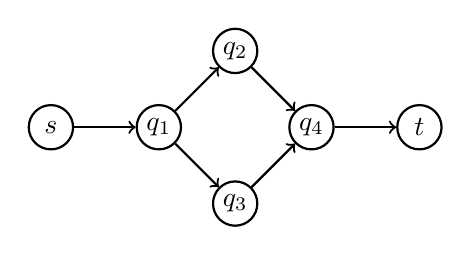
\begin{tikzpicture}[node distance={3.9em},
					thick, 
					main/.style = {draw, circle,fill=white, inner sep=1pt, minimum size=16pt}] 
					
					\node[main] (1) {$q_1$}; 
					\node[main] (2) [above right of=1] {$q_2$}; 
					\node[main] (3) [below right of=1] {$q_3$}; 
					\node[main] (4) [above right of=3] {$q_4$};
					\node[main] (5) [right of=4] {$t$}; 
					\node[main] (0) [left of=1] {$s$}; 
					\draw[->] (1) -- (2);
					\draw[->] (1) -- (3);
					\draw[->] (2) -- (4); 
					\draw[->] (3) -- (4); 
					\draw[->] (4) -- (5); 
					\draw[->] (0) -- (1);
				\end{tikzpicture}  
			\end{minipage}\hfill%
			\begin{minipage}[c]{0.64\textwidth}
				\begin{tikzpicture}[
					node distance={5.8em}, thick, 
					main/.style = {draw, rectangle, rounded corners=0.05cm,
						blur shadow, fill=white, inner sep=2pt, minimum size=13pt}
					]
					
					\node[main] (q1_eps) {$(q_1, \varepsilon)$}; 
					\node[main, fill=gray!30] (q1_b) [below right of=q1_eps] {$(q_1,b)$};
					
					\node[main] (q2_eps) [above right of=q1_eps]  {$(q_2,\varepsilon)$}; 
					\node[main, fill=gray!30] (q2_b) [below right of=q2_eps] {$(q_2,b)$};
					
					\node[main] (q3_eps) [below right of=q1_b] {$(q_3,\varepsilon)$}; 
					\node[main, fill=gray!30] (q3_b) [below right of=q3_eps] {$(q_3,b)$};
					
					\node[main] (q4_eps) [above right of=q3_eps] {$(q_4,\varepsilon)$};
					\node[main, fill=gray!30] (q4_b) [below right of=q4_eps] {$(q_4,b)$};
					
					\node[main, above right of=q4_eps] (t_eps) {$(t,\varepsilon)$};
					\node[main] (s_eps) [left of=q1_eps, xshift=0.3cm] {$(s,\varepsilon)$};
					
					\path[->] 
					(q1_eps)  edge [below,pos=.3] node {$b$} (q1_b)
					(q1_eps)  edge [left] node {$a$} (q2_eps)
					(q1_b)    edge [below,pos=.3] node {$a$} (q3_eps)
					(q1_b)    edge [out=180,in=290,above] node {$b$} (s_eps);
					
					\path[->] 
					(q2_eps) edge [out=280,in=175,below] node {$a$} (q4_eps)
					(q2_eps) edge [above,pos=.6] node {$b$} (q2_b)
					(q2_b)   edge [above,pos=.6] node {$a$} (q4_eps);
					
					\path[->] 
					(q4_eps) edge [left] node {$a$} (t_eps)
					(q4_eps) edge [left,pos=.5] node {$b$} (q4_b)
					(q4_b)   edge [left] node {$a$} (t_eps);
					
					% Koordinaten für Rücksprünge
					\coordinate (C) at ($(q4_b)+(0,-1.8)$);
					\coordinate (D) at ($(q2_b)+(0,1.8)$);
					
					\draw[->, rounded corners] 
					(q2_b) -- (D) -- (s_eps |- D) node[midway, above] {$b$} -- (s_eps);
					
					\draw[->, rounded corners] 
					(q4_b) -- (C) -- (s_eps |- C) node[midway, above] {$b$} -- (s_eps);
					
					\path[->] 
					(q3_eps) edge [above,pos=0.3] node {$a$} (q4_eps)
					(q3_eps) edge [below,pos=0.3] node {$b$} (q3_b)
					(q3_b)   edge [left] node {$a$} (q4_eps)
					(q3_b)   edge [out=180,in=280,above] node {$b$} (s_eps);
					
					\path[->] 
					(s_eps) edge node [above] {$a$} (q1_eps)
					(s_eps) edge [out=140, in=120, looseness=8, above] node {$b$} (s_eps);
					
					\path[->] 
					(t_eps) edge [loop above] node {$a,b$} (t_eps);
				\end{tikzpicture}
			\end{minipage}
			\caption[Example for reduction used in the proof of Prop.~\ref{prelim:prop:sync_NL_complete}]{Example for the reduction used in \cref{prelim:prop:sync_NL_complete}. Left: Input graph. Right: Transformation into an automaton having a synchronizing word if and only if there exists a path from $s$ to $t$ in the input graph (states from $V \times \{b\}$ are colored grey).}
			\label{prelim:fig:sync_NL_hard}
		\end{figure}
	
	\medskip 
	\noindent\underline{Properties:} The following two properties are readily seen.
	\begin{enumerate}
		\item \label{prelim:synctrap:bb} 
		$\applytrans{\delta}{Q \setminus \{(t,\varepsilon)\}}{bb} = \{(s,\varepsilon)\}$
		and  $\applytrans{\delta}{(t, \varepsilon)}{bb} = (t,\varepsilon)$.		
		
		\item \label{prelim:synctrap:transition} For $q \in V \setminus \{s,t\}$ 
		we have $\applytrans{\delta}{(q, \varepsilon)}{a} = (q^R,\varepsilon)$
		and $\applytrans{\delta}{(q, \varepsilon)}{ba} = (q^L,\varepsilon)$.
	\end{enumerate}
	
	\medskip 
	\noindent\underline{Verification:} First, suppose there exists a path $q_0, q_1, \ldots, q_n$
	with $q_0 = s$ and $q_n = t$ in $G$.
	Define a word $u = u_1 u_2 \cdots u_n$ 
	where $u_1 = a$ and, for $i \in \{2,\ldots,n\}$, 
	\[
	u_i = \begin{cases}
		a   & \text{if } q_i = q_{i-1}^R, \\
		ba	& \text{if } q_{i-1}^R \ne q_{i-1}^L \text{ and } q_i = q_{i-1}^L. 	
	\end{cases}
	\]	
	By Properties~\ref{prelim:synctrap:bb} and~\ref{prelim:synctrap:transition}, 
	$\applytrans{\delta}{Q}{bbu_1 \cdots u_i} = \{ (q_i,\varepsilon), (t,\varepsilon) \}$.
	So $\delta(Q,bbu) = \{(t,\varepsilon)\}$.		
	
	Conversely, suppose the word $u \in \Sigma^*$
	synchronizes $\mathcal A$.
	As $(t,\varepsilon)$ is a trap state, we have $\applytrans{\delta}{Q}{u} = \{(t,\varepsilon)\}$.
	Let $w$ be a shortest factor of $u$ such that $\delta((s,\varepsilon), w) = (t,\varepsilon)$.
	By Property~\ref{prelim:synctrap:bb} we have $w \notin \Sigma^* bb \Sigma^*$, i.e., 
	$w \in \{a,ba\}^* \cup \{a,ba\}^*b$.
	As we can enter the state $(t,\varepsilon)$ from another state only via the letter~$a$,
	we have $w \in \{a,ba\}^*$. 
	Let $w = w_1 \cdots w_n$ with 
	$w_1, \ldots, w_n \in \{a,ba\}^*$.
	Then, by Property~\ref{prelim:synctrap:transition}, the vertices
	\[
	(s,\varepsilon), \applytrans{\delta}{s}{w_1}, \applytrans{\delta}{s}{w_1 w_2} \ldots
	\applytrans{\delta}{s}{w_1 w_2\cdots w_{n-1}}, (t,\varepsilon) 
	\]
	trace out a path in $G$ from $s$ to $t$.		
\end{proof} 

\begin{proposition}\label{prelim:complexity:prop:maximum}
	Given an automaton $\semiautomat{A}{Q}{\Sigma}{\delta}$ and $q \in Q$
	it is \NL-complete to test whether $q$ is a maximum w.r.t.~the 
	reachability quasiorder $\lereach$.	
\end{proposition}
\begin{proof}
	First, we give
	an $\leACZEROm$-reduction from \DFAST, which yields \NL-hardness by \PROP~\ref{prelim:prop:sync_NL_complete}.
	Let $\semiautomat{A}{Q}{\Sigma}{\delta}$
	be an input instance to \DFAST.
	Suppose $t \in Q$ is the trap state, which 
	can be computed by an $\AC^0$-circuit as 
	in the proof of \crefitem{compl:prop:reductions}{compl:prop:reductions:item:st-ss}.
	So, the reduction produces $\mathcal A$ together with the trap state~$t$
	and $(\mathcal A, t)$ is a {\sc Yes}-instance of our problem
	if and only if $\mathcal A$ is synchronizing,
	since the state $t$ is a maximum in $\mathcal A$
	if and only if~$\mathcal A$ is synchronizing by \cref{prelim:thm:sync_trap_state}.
		
	For containment in \NL, suppose $\semiautomat{A}{Q}{\Sigma}{\delta}$ and $q \in Q$
	are given.
	To test whether $q$ is a maximum for $\lereach$,
	we guess, for each state $p \in Q$,
	a word $u \in \Sigma^{<|Q|}$
	letter by letter and check whether $\applytrans{\delta}{p}{u} = q$; a property that characterizes that~$q$ is a maximum
	by \cref{prelim:classes:sync:cor:sync-state}.
	This can be 
	done in nondeterministic log-space
	by storing a state
	and using two counters, one to iterate through all states $p \in Q$
	and the other to make at most $|Q|$ guessing steps for each $p \in Q$.	
\end{proof}

\begin{proposition}\label{prelim:complexity:prop:maximal}
	Given an automaton $\semiautomat{A}{Q}{\Sigma}{\delta}$ and $q \in Q$
	it is \NL-complete to test whether $q$ is maximal w.r.t.~the 
	reachability quasiorder $\lereach$.	
\end{proposition}
\begin{proof}
	We give a reduction
	from the \NL-complete problem \TWODAGST.
	Let $G = (V, E)$ and $s, t \in V$ be an input instance.
	Construct an automaton $\semiautomat{A}{Q}{\Sigma}{\delta}$
	as in the proof of \cref{prelim:prop:sync_NL_complete},
	but instead of making $(t,\varepsilon)$ a trap state,
	let both letters $a$ and $b$ map back to the state $(s,\varepsilon)$.
	Then $t$ is a maximal state (and~$\mathcal A$
	is strongly connected) if and only if there exists
	a path from~$s$ to $t$ in~$G$.
		
	To test maximality, we have to check
	that for each state $p \in Q$
	with $\delta(q, u) = p$ for some $u \in \Sigma^*$
	there exists $v \in \Sigma^*$
	with $\delta(p, v) = q$.
	To verify this condition, we can pick words $u,v$
	of length at most $|Q|$
	and proceed similarly as in the proof of \cref{prelim:complexity:prop:maximum}
	to obtain \NL-membership.	
\end{proof}

Similar procedures as in \cref{prelim:complexity:prop:maximum,prelim:complexity:prop:maximal}
can be used to check whether a state is minimal or a minimum, but we do not need to check these properties
in the following and hence give no formal statement. We also note that we obtain
\LOGSPACE-completeness of these problems in case the input automata are unary automata
since we only needed nondeterminism when guessing different letters in the above proofs.

\begin{theorem}\label{prelim:complexity:general_aut_sync}
	The problems \DFAS, \DFAST and \DFASS
	are \NL-complete, even for a fixed binary alphabet.
\end{theorem}
\begin{proof} 
	By Proposition~\ref{compl:prop:reductions} 
	we have $\DFAST \leACZEROm \DFASS$
	and $\DFAST \leACZEROm \DFAS$.
	By \cref{prelim:prop:sync_NL_complete}, \DFAST\   %can be solved by an \NL-algorithm % fussnote alternative paare auf q
	is \NL-hard for an alphabet containing at least two letters.
	\DFAS\ is in \NL, see \cref{compl:sec:subclasses:known-results} (page~\pageref{prelim:classes:intro:SYNC}).
	For $\semiautomat{A}{Q}{\Sigma}{\delta}$, by \THM~\ref{prelim:thm:SCC_sync_words},
	a state $q \in Q$
	is a synchronizing state if and only if $\mathcal A$ is synchronizing and $q$ is
	a maximum for the reachability order $\lereach$.
	The latter two properties can be checked in \NL\  since \DFAS\ is in \NL and by~\cref{prelim:complexity:prop:maximum}, respectively.
	So, \DFASS is in~\NL.	
\end{proof}

\begin{proposition}\label{prelim:thm:ST-PSPACE}
	\ST is in \PSPACE.
\end{proposition}
\begin{proof}
	Let $(\mathcal A, S, T)$ with $\semiautomat{A}{Q}{\Sigma}{\delta}$
	and $S, T \subseteq Q$ where $S = \{s_1, \ldots, s_m\}$ and $n = |Q|$.
	Store the values $s_1, \ldots, s_m$ in $m$ memory cells
	and then repeat the following steps
	at most~$n^m$ times:  
	If the memory cells store a subset of~$T$, then abort and return \rYES, i.e., classify 
	this input instance as a \rYES-instance of the decision problem.
	Otherwise
	guess a letter $a \in \Sigma$ and update the memory cells
	with $\applytrans{\delta}{s_1}{a}, \ldots, \applytrans{\delta}{s_m}{a}$.
	If this procedure finishes without ever writing a subset of~$T$ into the memory cells, 
	then return \rNO.
	The upper bound for the number of steps
	can be ensured by utilizing an  $(m\cdot \log n)$-bit counter 
	counting the number of steps in binary encoding.
	After at most $n^m$
	steps we have seen at least one memory cell configuration twice.
	So, if there exists a word mapping $S$ into $T$, then
	there exists such a word of length at most $n^m$,
	which implies correctness of the algorithm.
	As it runs in nondeterministic polynomial space,
	and as \PSPACE\  = \NPSPACE\ by Savitch's theorem~\cite{DBLP:journals/jcss/Savitch70},
	the claim follows.
\end{proof}

The following lemma is a technical result that we need to reduce an arbitrary alphabet to a binary alphabet
in our subset mapping problems.
Another reduction to reduce the alphabet for synchronization problems has been given
in~\cite[Sec.~5]{Martyugin12} and~\cite[Prop.~2]{Martyugin14}.


\begin{lemma} \label{prelim:lem:alphabet-reduction}
	Let $\semiautomat{A}{Q}{\Sigma}{\delta}$ with $\Sigma = \{a_1, \ldots, a_k\}$.
	Set $C = \{ 0^{k} 10^i1 \mid i \in \{0,1,\ldots,k-1\}\}$
	and $\semiautomat{B}{Q \times \pref{C}\setminus C}{\{a,b\}}{\mu}$
	where, for $q \in Q$, $u \in \pref{C}\setminus C$, and $x \in \{a,b\}$,
	we have
	\[
	\mu((q,u), x) =
	\begin{cases}
		(\delta(q, a_i), \varepsilon) & \text{if } ux = 0^k10^{i-1}1 \text{ for some } i \in \{1,\ldots,k\}, \\
		(q, ux)  & \text{if } ux \in \pref{C} \setminus C, \\
		(q, ux)  & \text{if } u \in \pref{0^{k-1}} \text{ and } x = 0, \\
		(q, 0^k) & \text{if } u = 0^k \text{ and } x = 0, \\
		(q, 0^k) & \text{if } u = 0^k10^{k-1} \text{ and } x = 0, \\
		(q, \varepsilon) & \text{otherwise.}
	\end{cases}
	\]
	Then $\mathcal A$ is strongly connected if and only if $\mathcal B$ 
	is strongly connected and, for $i \in \{1,\ldots,k\}$, $q \in Q$, $u \in \pref{C}\setminus C$,
	we have
	\begin{equation}\label{prelim:eqn:general-to-binary}
	\mu((q, u), 0^k10^{i-1}1) = (\delta(q, a_i), \varepsilon),
	\end{equation}
	and, for distinct $S, T \subseteq Q$,
	we have $\delta(S, u) = T$ for some $u \in \Sigma^*$
	if and only if $\mu(S \times \pref{C}\setminus C, v) = T \times \{\varepsilon\}$ 
	for some $u \in \{a,b\}^*$.
\end{lemma}
\begin{proof}
	That~$\mathcal A$ is strongly connected if and only if~$\mathcal B$
	is strongly connected is easy to see.
	\Cref{prelim:eqn:general-to-binary} is also easy to verify.
		
 Next, suppose $\delta(S, u) = T$ for some $u \in \Sigma^*$. Since $S \ne T$ we have $|u| > 0$.
 Let $v_j = 0^k 1 0^{i-1} 1$ if the $j$-th symbol in~$u$ equals $a_i$
 for $i \in \{1,\ldots,k\}$.
 By \cref{prelim:eqn:general-to-binary} 
 we have $\mu(S \times \pref{C}\setminus C, v_1 \cdots v_{|u|}) = (T, \varepsilon)$.
 
 Conversely, suppose $\mu(S \times \pref{C}\setminus C, v) = T \times \{\varepsilon\}$ 
 for some $u \in \{a,b\}^*$.
 Let $q \in S$ and $u \in \pref{C}\setminus C$.
 The language~$C$ has the property that there exist unique words
 $u_1, \ldots, u_m \in C$ and $v_0, \ldots, v_m \in \Sigma^*$,
 each $v_j$ containing no factor from~$C$, such that
 \[
 uv = v_0 u_1 v_1 \cdots u_m v_m.
 \]
 For each $j \in \{1,\ldots,m\}$, set $x_j=a_i$ if
 $u_j = 0^k10^{i-1}1$ for some $i \in \{1,\ldots,k\}$.
 By induction, using \cref{prelim:eqn:general-to-binary}, we obtain
 \[
 \mu((q,u),v)
 =
 (\delta(q,x_1\cdots x_m),\varepsilon).
 \]
 Hence $\delta(S,x_1\cdots x_m)=T$. 
\end{proof}

\begin{theorem}\label{prelim:thm:binary_pspace_problems} The following problems are \PSPACE-complete w.r.t.~$\lelogm$-reductions:
	\begin{enumerate}
		\item \SFS and \SIS even on binary strongly connected  automata,
		\item \DFAINT, \ST, and \DST even on binary strongly connected  automata,
		\item \REACH and \REACHF even for binary automata.
	\end{enumerate}
\end{theorem}
\begin{proof}
	Membership of these problems in \PSPACE\ was 
	proved in the literature, see  \cref{compl:sec:subclasses:known-results} (page~\pageref{prelim:classes:intro:SFS}).
	As an example, we included a proof
	for \ST in \cref{prelim:thm:ST-PSPACE}.
	
	\PSPACE-hardness of \SFS and \SIS for binary strongly connected automata
	was also mentioned  in \cref{compl:sec:subclasses:known-results} (page~\pageref{prelim:classes:intro:SFS}).
	
	By \cref{compl:prop:reductions} we have
	\[
	\SIS \leACZEROm \ST \leACZEROm \DFAINT
	\]
	and the reductions from \cref{compl:prop:reductions}
	preserve strong connectedness and the alphabet.
	Thus, the claim for \ST and \DFAINT follow.
	
	The reduction showing $\ST \leACZEROm \DFAINT$
	from \cref{compl:prop:reductions:item:DFAINT_ST} in \cref{compl:prop:reductions}
	does not preserve strong connectedness and the alphabet.
	However, it can easily be adapted 
	by adding a new letter that swaps two states $q$ and $(q,0)$ 
	with $q \in S$
	and induces a self-loop at every other state not in~$S$.
	Then the resulting automaton is strongly connected
	and this gives a valid reduction.
	With \cref{prelim:lem:alphabet-reduction} 
	we then obtain \PSPACE-hardness
	even for binary strongly connected automata.
	This proves the claim for \DFAINT, \ST, and \DST.
	
	\REACH was shown to be \PSPACE-hard
	in~\cite[Thm.~3.2]{Rys83}
	and~\cite[Thm.~3]{BondarV16}
	by reductions from  
	\SIS and \DFAINT, respectively,
	that add a single new letter.
	Neither of these reductions preserves strong connectedness.
	By \cref{prelim:lem:alphabet-reduction}	we obtain a reduction 
	to a binary alphabet.
	Since $\REACH \leACZEROm \REACHF$
	by \cref{compl:prop:reductions}
	where the reduction preserves the alphabet,
	we obtain the hardness claims for \REACH and \REACHF.
\end{proof}